%======================================================================
%  Anexo E - Diagramas del modulo en notacion de Chen (draw.io)
%======================================================================

\section{Diagramas del módulo en notación de Chen}
\label{anx:chen}

En el cuerpo del documento los diagramas del módulo se presentan como
quedaron en Oracle SQL Developer Data Modeler. Este anexo conserva las
versiones elaboradas en draw.io con la notación de Chen, que muestran lo que la notación
Barker de la herramienta omite: el nombre de cada relación, su
participación (mín,máx) y, en el modelo relacional, la tabla a la que
apunta cada clave foránea. Ambas versiones representan el mismo modelo y
se verificaron entre sí relación por relación.

La figura~\ref{fig:vistaU4chen} corresponde a la vista U4 del mensajero
(figura~\ref{fig:vistaU4}); en ella la asignación de un envío a un
despacho es la relación N:M \textit{contiene}, con los atributos orden de
visita y resultado.

{\singlespacing
\begin{figure}[!htb]
\centering
\adjustbox{max width=\linewidth, max totalheight=0.42\textheight}{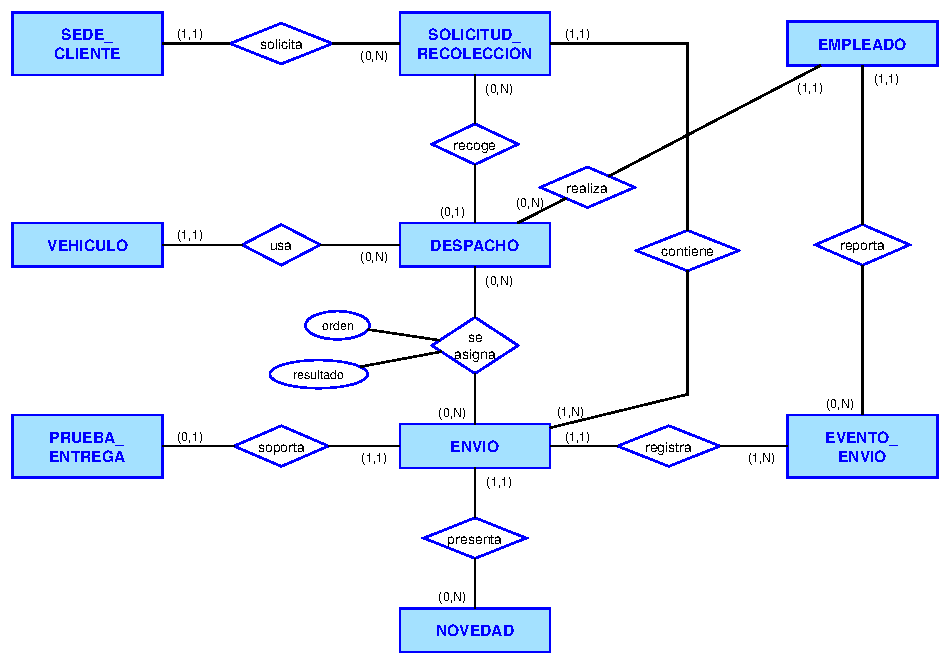
\includegraphics{figuras/er/M_U4.pdf}}
\caption{Vista U4: mensajero, en notación de Chen.}
\label{fig:vistaU4chen}
\end{figure}
\par}

La figura~\ref{fig:erfinal} es el modelo Entidad-Relación ajustado del
módulo (figura~\ref{fig:dmlogico}): 19 entidades, 26 relaciones con
nombre y la especialización parcial de EMPLEADO en MENSAJERO.

La figura~\ref{fig:relacional} es el modelo relacional del módulo
(figura~\ref{fig:dmrelacional}). En cada tabla, \texttt{P} marca la
clave primaria, \texttt{F} una clave foránea (con la tabla a la que
apunta), \texttt{PF} una columna que es ambas, \texttt{U} un valor
único, \texttt{*} una columna obligatoria y \texttt{o} una opcional.

\begin{landscape}
{\singlespacing
\begin{figure}[p]
\centering
\adjustbox{max width=22.5cm, max totalheight=14.6cm}{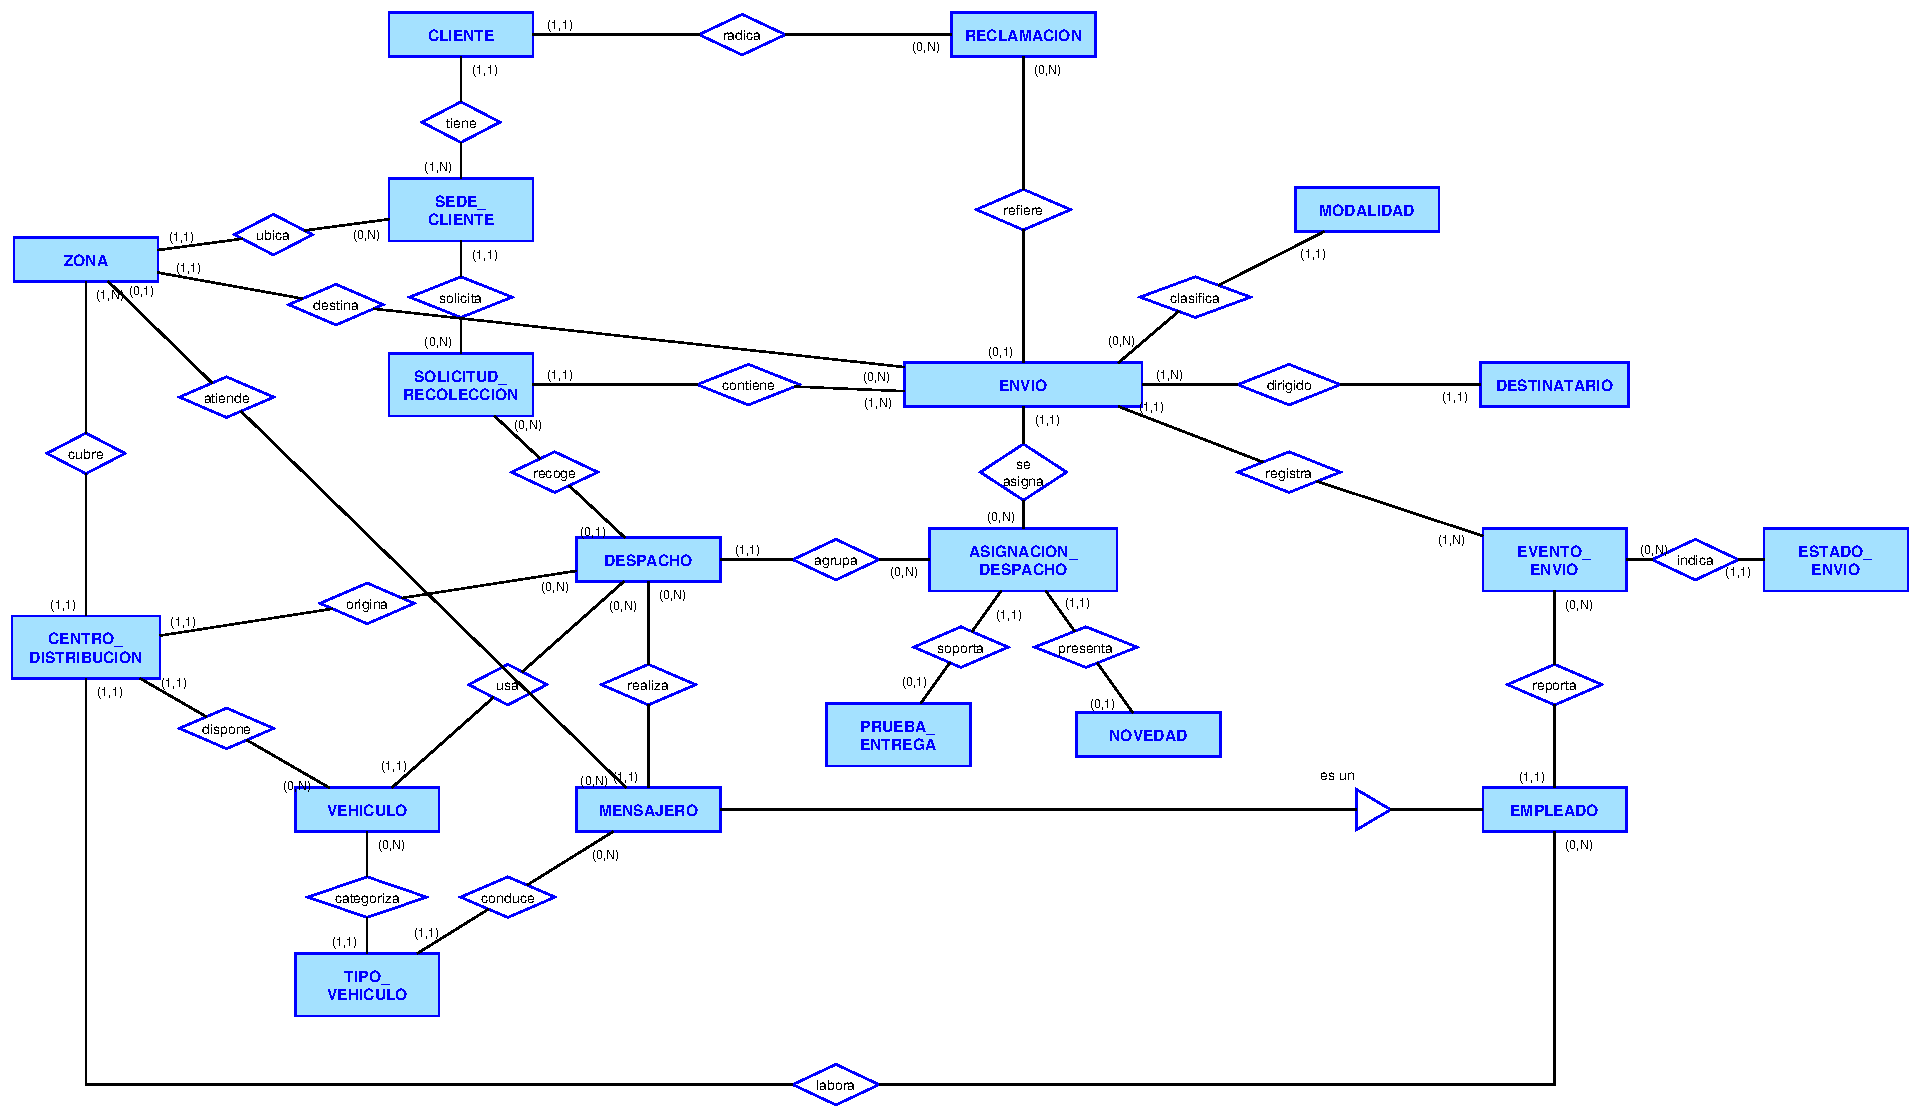
\includegraphics{figuras/er/M_final.pdf}}
\caption{Modelo Entidad-Relación ajustado del módulo de operación de envíos, en notación de Chen.}
\label{fig:erfinal}
\end{figure}
\par}
\end{landscape}

\begin{landscape}
{\singlespacing
\begin{figure}[p]
\centering
\adjustbox{max width=22.5cm, max totalheight=14.6cm}{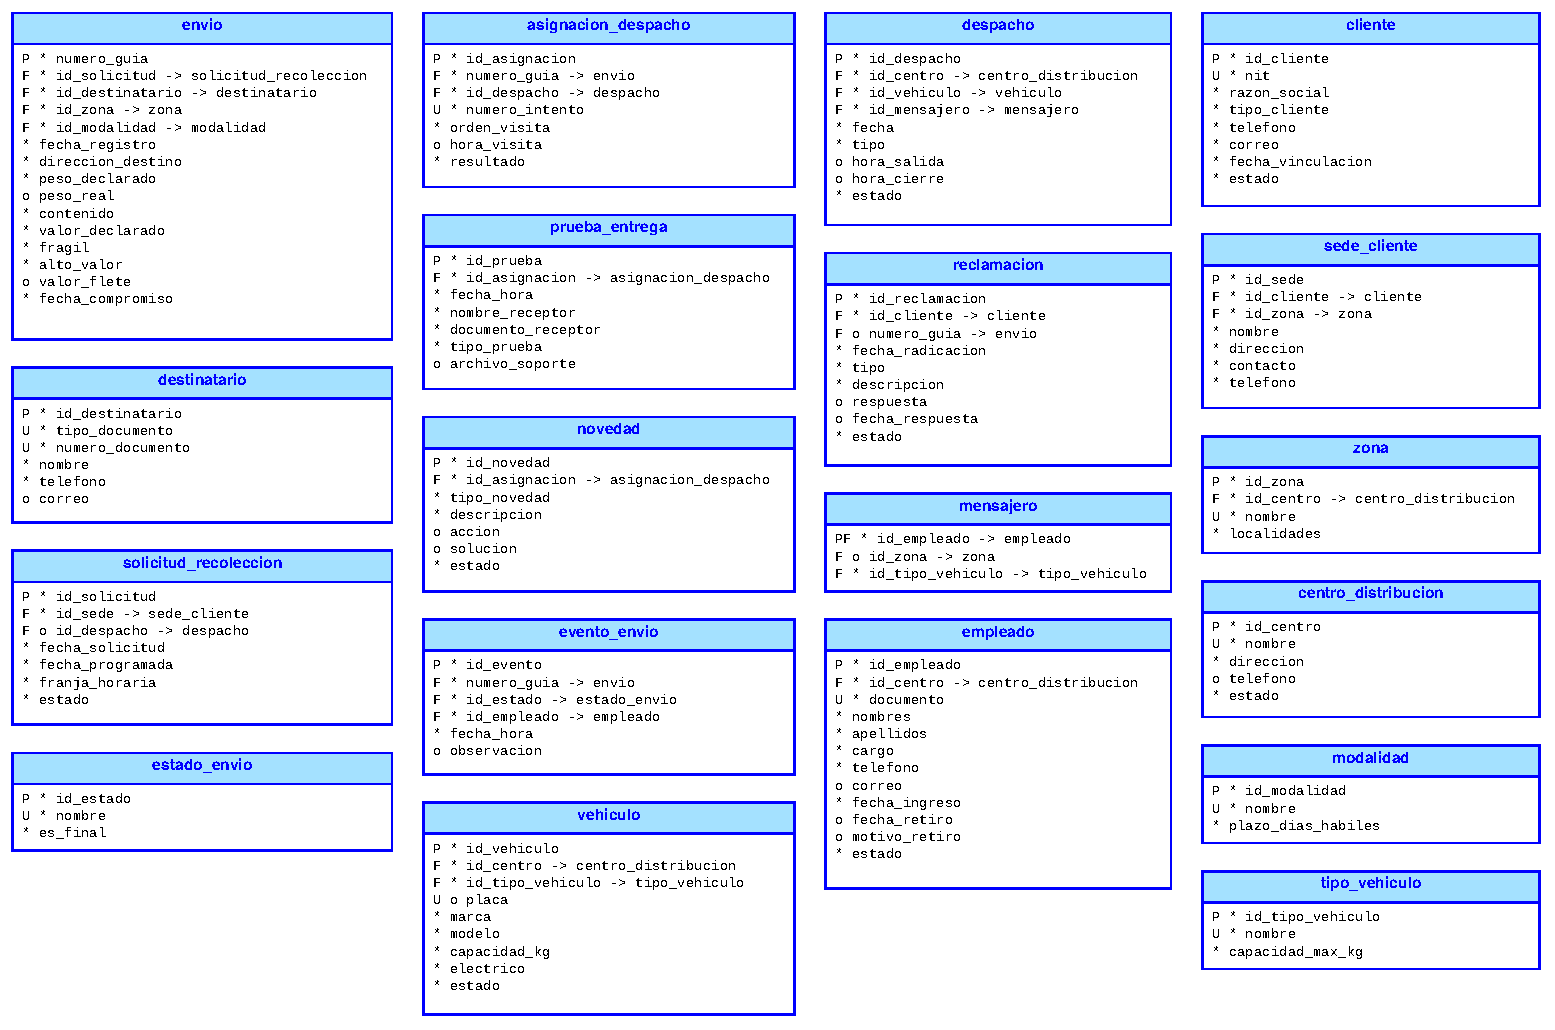
\includegraphics{figuras/er/M_relacional.pdf}}
\caption{Modelo relacional del módulo de operación de envíos, elaborado en draw.io.}
\label{fig:relacional}
\end{figure}
\par}
\end{landscape}
